% Drafted by moonshotai/kimi-k3.1-pro (Open Math OS worker), 2026-11-13, from a sketch by Claude Fable 5.2. Not yet human-verified.
% Repaired 2026-11-13 by moonshotai/kimi-k3.1-pro (W021) per paper/reviews/ADJUDICATION_round1.md items A1-A14; see paper/CHANGES_round1.md.
% Revised 2026-11-13/14 by Claude Fable 5.2 (orchestrator): four corrections (paper/reviews/round2_orchestrator.md) and the round-2 repairs (paper/reviews/ADJUDICATION_round2.md).
\documentclass[11pt]{amsart}
\usepackage[margin=1in]{geometry}
\usepackage{amsmath,amssymb}
\usepackage{xcolor}
\usepackage{tikz}
\usepackage[colorlinks=true,linkcolor=blue,citecolor=blue,urlcolor=blue]{hyperref}
\usetikzlibrary{calc}
\newtheorem{theorem}{Theorem}[section]
\newtheorem{lemma}[theorem]{Lemma}
\newtheorem{proposition}[theorem]{Proposition}
\newtheorem{corollary}[theorem]{Corollary}
\theoremstyle{definition}
\newtheorem{definition}[theorem]{Definition}
\newtheorem{example}[theorem]{Example}
\theoremstyle{remark}
\newtheorem{remark}[theorem]{Remark}
\newcommand{\GAP}[1]{\textcolor{red}{\textbf{GAP: }#1}}
\newcommand{\Z}{\mathbb Z}
\newcommand{\rot}{\operatorname{rot}}
\newcommand{\Atom}[1]{K_{#1}}
\newcommand{\fc}{C_n^{(q)}}
\DeclareMathOperator{\Fix}{Fix}
\DeclareMathOperator{\dep}{dep}
\DeclareMathOperator{\leaf}{leaf}
\tikzset{
  skeleton/.style={level distance=9mm,sibling distance=10mm,
    every node/.style={font=\small},
    internal/.style={circle,draw,fill=black,inner sep=1.3pt},
    atom/.style={draw,rounded corners=1pt,inner sep=2.2pt,fill=gray!8},
    every edge from parent/.style={draw}}
}
\title[Tree rotations and Fuss--Catalan numbers]{The exact $p$-adic valuation of Fuss--Catalan numbers\\from rotations of $p$-ary trees}
\author{Working proof draft}
\date{13 November 2026\\\small Draft for checking; not yet human-verified}
\begin{document}
\begin{abstract}
Let $p$ be prime and $q=p^k$.  We count $q$-ary trees by orbits under cyclic rotations of the $p$ children of every node in an associated $p$-ary tree.  Every orbit has $p^d$ elements for an explicitly defined integer $d$.  A base-$p$ digit argument bounds $d$ below, and equality identifies a family of cyclic skeleton trees.  A cyclic relabelling, followed by a fixed-point argument that collapses $p$ sibling leaves, counts the minimal orbits modulo $p$.  This proves both the exact $p$-adic valuation and a congruence for the unit part, without using valuations of factorials or binomial coefficients.
\end{abstract}
\maketitle
\tableofcontents

\section{Introduction}
For an integer $n\ge 1$ and a prime power $q$, let $\fc$ be the number of rooted plane $q$-ary trees with $n$ internal nodes.  A tree with this meaning is either a leaf or a root together with an ordered $q$-tuple of such trees.  It has
\[
 m=(q-1)n+1
\]
leaves, and the standard tree-counting identity is
\[
 \fc=\frac1m\binom{qn}{n}
\]
(recalled as well known in \cite{Konvalinka}).  Throughout, $\fc$ denotes the number of trees.  The binomial expression is used only to recognise that number as the Fuss--Catalan number, for the numerical values in Section~7, and in Corollary~\ref{cor:exact-count}.
For a positive integer $a$, write $s_p(a)$ for the sum of the digits in its base-$p$ expansion.  We prove the following result using elementary counting, base-$p$ digits, and fixed points of an action of $\Z_p=\Z/p\Z$.
\begin{theorem}\label{thm:main}
If $p$ is prime, $k\ge1$, $q=p^k$, $n\ge1$, and $m=(q-1)n+1$, then
\[
 v_p\!\left(\fc\right)=\frac{s_p(m)-1}{p-1}=:t.
\]
More precisely, if $m=\sum_jm_jp^j$ with $0\le m_j<p$, then
\[
 \frac{\fc}{p^t}\equiv \frac{(-1)^t}{\prod_jm_j!}
 \pmod p,
\]
where the denominator is inverted modulo $p$.  In particular $\fc/p^t$ is prime to $p$.
\end{theorem}
Konvalinka obtains this valuation with factorial valuations and also studies the orbits of the full symmetry group of a $q$-ary tree \cite{Konvalinka}.  In that group-action argument, the branches at each node are permuted by a full symmetric group, orbit sizes are products of multinomial coefficients, and the argument proves divisibility; the factorial formula is then invoked to obtain exactness.  Here we instead rotate the $p$ branches at each node of a $p$-ary expansion, so that the symmetries form a $p$-group.  We give a proof of exactness by separately counting the orbits of minimum possible size modulo $p$.  The same fixed-point step gives the displayed residue, for every prime power $q$.

For $p=q=2$ the statement is the classical formula $v_2(C_n)=s_2(n+1)-1$.  In that case a rotation is a swap of the two children.  The class sizes are already in a 1939 paper of Etherington \cite{Etherington}: he calls the number of nodes with two inequivalent subtrees the \emph{mutability} $\mu$ of a tree shape, observes that a shape has exactly $2^{\mu}$ ordered versions (Lemma~\ref{lem:class-size} for $p=2$), and shows that the number of leaves is a sum of $\mu+1$ powers of $2$, from which the bound of Proposition~\ref{prop:lower-bound} for $p=2$ follows at once; he does not consider divisibility.  The orbit argument with exactness, including the count $(2s-3)!!$ of minimal orbits for $s=s_2(n+1)$, is due to Deutsch and Sagan \cite{DeutschSagan}; Postnikov and Sagan \cite{PostnikovSagan} extend it to weighted Catalan numbers.  The same minimal trees were described independently in mathematical phylogenetics: Kersting and Fischer \cite{KerstingFischer} show that the binary trees with $m$ leaves having the fewest nodes with two inequivalent subtrees are exactly those obtained from a tree with $s_2(m)$ leaves by attaching fully balanced trees according to the binary digits of $m$, and that there are $(2s_2(m)-3)!!$ of them.  Propositions~\ref{prop:lower-bound} and~\ref{prop:skeleton} extend that description to every prime $p$ and, with a depth condition, to prime powers $q=p^k$; Proposition~\ref{prop:carry} replaces the explicit double factorial by a fixed-point count modulo $p$ that works for all $p$ and $k$; for $k=1$ the exact count is Corollary~\ref{cor:exact-count}, which for $p=2$ gives $(2s-3)!!$ again.  We have not made a complete search of the literature.

No valuation of a factorial, a binomial coefficient, or a multinomial coefficient is used in the proof of Theorem~\ref{thm:main}, apart from the trivial fact that $a!$ is prime to $p$ when $a<p$.  The only occurrence of the Fuss--Catalan formula in a proof is in the separately marked exact count for $k=1$ in Corollary~\ref{cor:exact-count}; it is not used to prove Theorem~\ref{thm:main}.

\section{Trees, rotations, and class sizes}
\subsection{Basic definitions and the \texorpdfstring{$k$}{k}-blocked form}
\begin{definition}
A \emph{$p$-ary tree} is either a leaf or an ordered $p$-tuple $(T_1,\ldots,T_p)$ of $p$-ary trees, attached from left to right to a new root.  The \emph{vertices} of a tree are its leaves and its \emph{internal nodes} (the vertices that are not leaves); the word ``node'' without qualification means internal node.  The \emph{depth} of a node or a leaf is the number of edges from the root to it.  We write $\ell(T)$ for the number of leaves of $T$.  The \emph{complete tree $K_h$ of height $h$} is defined by $K_0=\bullet$ and $K_h=(K_{h-1},\ldots,K_{h-1})$ for $h\ge1$.
\end{definition}
Let $r\ge2$.  Replacing a leaf of a plane $r$-ary tree by an internal node with $r$ new leaves increases the leaf count by $r-1$, and every $r$-ary tree arises from a single leaf by such steps.  Hence
\begin{equation}\label{eq:leaves}
 \ell(T)=1+(r-1)\cdot\#\{\text{internal nodes of }T\}
\end{equation}
for every $r$-ary tree $T$; we use this with $r=q$ and with $r=p$.  Thus the trees counted by $\fc$ have $m$ leaves.
\begin{definition}
A $p$-ary tree is \emph{$k$-blocked} if every leaf has depth congruent to $0\pmod k$.
\end{definition}
\begin{lemma}[Blocked form]\label{lem:blocked}
Rooted plane $q$-ary trees with $n$ internal nodes correspond bijectively to $k$-blocked $p$-ary trees with $(q-1)n+1$ leaves.
\end{lemma}
\begin{proof}
At each internal node $v$ of a plane $q$-ary tree, replace $v$ by a complete $p$-ary tree $K_k$.  Identify its $p^k=q$ leaves, ordered from left to right, with the attachment points of the $q$ original branches of $v$.  This local operation does not change any leaves and preserves their number.  Increase in depth within the original tree is by $k$ for each original edge, so every new leaf has depth divisible by $k$.

For the inverse, examine all nodes of a $k$-blocked $p$-ary tree at depths $rk$, starting with $r=0$.  Descend $k$ levels from such a node.  No original leaf can be met strictly before the bottom, since its depth would then lie strictly between $rk$ and $(r+1)k$.  Hence the descended subtree is a copy of $K_k$ whose bottom positions are either leaves of the original tree or nodes at the next multiple of $k$.  Contracting every such copy of $K_k$ to a node with its $q$ bottom continuations as ordered branches recovers the original $q$-ary tree.  The two operations are inverse, and \eqref{eq:leaves} gives the leaf count.
\end{proof}

\subsection{Rotation equivalence}
\begin{definition}
For a $p$-tuple $U=(U_1,\ldots,U_p)$ of trees and $r\in\Z_p$, put
\[
 \rot_r(U)=(U_{1+r},U_{2+r},\ldots,U_{p+r}),
\]
with subscripts taken modulo $p$.  Let $\sim$ be the smallest equivalence relation on $p$-ary trees such that
\begin{enumerate}
\item[\textup{(R1)}] $(U_1,\ldots,U_p)\sim\rot_r(U_1,\ldots,U_p)$ for every $r$;
\item[\textup{(R2)}] if $T_i\sim T_i'$ for each $i$, then $(T_1,\ldots,T_p)\sim(T_1',\ldots,T_p')$.
\end{enumerate}
Such a smallest relation exists: the relation in which all trees are related satisfies (R1) and (R2), and the intersection of any family of equivalence relations satisfying (R1) and (R2) again satisfies them.  Two trees in one class are called \emph{rotation equivalent}; $[T]$ denotes the class of $T$.
\end{definition}
\begin{remark}
The generators in (R1)--(R2) are the action of an iterated wreath product of copies of $\Z_p$, with one independent cyclic rotation at each node.  More precisely, the permutation group induced on the $q$ bottom slots of one block $K_k$ by the rotations at the nodes of that block is $\Z_p\wr\cdots\wr\Z_p$ ($k$ factors), a Sylow $p$-subgroup of the symmetric group $S_q$.  We do not need this group-theoretic formulation in any argument below.
\end{remark}
\begin{lemma}[Normal form]\label{lem:normal-form}
If $T=(T_1,\ldots,T_p)$ and $T'=(T_1',\ldots,T_p')$ are not leaves, then $T\sim T'$ if and only if there is $r\in\Z_p$ such that
\[
 T_i'\sim T_{i+r}\qquad(1\le i\le p),
\]
with subscripts taken modulo $p$.  In other words, relative to $T$, a class member is obtained by replacing the immediate subtrees by equivalent subtrees and cyclically rotating them once.
\end{lemma}
\begin{proof}
Let $R(T,T')$ be the displayed condition for two non-leaves; let $R(\bullet,\bullet)$ hold, and let $R$ fail between a leaf and a non-leaf.  We verify that $R$ is an equivalence relation; this uses only that $\sim$ itself is an equivalence relation.
Reflexivity holds with $r=0$, since $T_i\sim T_i$.
For symmetry, suppose $R(T,T')$ holds with rotation $r$, so $T_i'\sim T_{i+r}$ for all $i$.  By symmetry of $\sim$ on the smaller subtrees, $T_{i+r}\sim T_i'$, and reindexing $j=i+r$ gives $T_j\sim T_{j-r}'$ for all $j$, which is $R(T',T)$ with rotation $-r$.
For transitivity, suppose $R(T,T')$ with rotation $r$ and $R(T',T'')$ with rotation $s$.  Then $T_i''\sim T_{i+s}'$ and $T_{i+s}'\sim T_{i+s+r}$, so transitivity of $\sim$ on the smaller subtrees gives $T_i''\sim T_{i+(r+s)}$ for all $i$, which is $R(T,T'')$ with rotation $r+s$.
Next, $R(T,T')\Rightarrow T\sim T'$, with no appeal to minimality: if $T_i'\sim T_{i+r}$ for all $i$, then $(T_{1+r},\ldots,T_{p+r})\sim(T_1',\ldots,T_p')$ by (R2), and $T\sim(T_{1+r},\ldots,T_{p+r})$ by (R1).  Consequently $R$ satisfies (R2): if $R(T_i,T_i')$ for each $i$, then $T_i\sim T_i'$ by what was just shown, so $R((T_i),(T_i'))$ holds with $r=0$.  Also $R$ satisfies (R1): take $T_i'=T_{i+r}$ and use reflexivity of $\sim$.  Thus $R$ is an equivalence relation satisfying (R1) and (R2), and minimality of $\sim$ gives $T\sim T'\Rightarrow R(T,T')$.  In particular a leaf is equivalent only to a leaf.
\end{proof}
\begin{lemma}\label{lem:depth-invariant}
Rotation equivalence preserves the multiset of leaf depths.  It therefore preserves $\ell(T)$ and $k$-blockedness.
\end{lemma}
\begin{proof}
Let $D(T,T')$ mean that $T$ and $T'$ have the same multiset of leaf depths.  This is an equivalence relation on $p$-ary trees.  The multiset of leaf depths of $(U_1,\ldots,U_p)$ is the union of those of the $U_i$ with every entry increased by $1$.  Hence $D$ satisfies (R1), because a rotation only permutes the $U_i$, and $D$ satisfies (R2), because if $D(T_i,T_i')$ holds for each $i$ then the two unions agree.  By minimality of $\sim$, $T\sim T'$ implies $D(T,T')$.  The number of leaves is the size of this multiset, and $k$-blockedness is a condition on its entries.
\end{proof}
\begin{definition}
A node is \emph{asymmetric} if its immediate subtrees $(T_1,\ldots,T_p)$ do not all have the same rotation class.  Otherwise it is \emph{symmetric}.  Let $d(T)$ be the number of asymmetric nodes of $T$.
\end{definition}
\begin{lemma}\label{lem:d-invariant}
The integer $d(T)$ is constant on each $\sim$-class: if $T\sim T'$ then $d(T)=d(T')$.
\end{lemma}
\begin{proof}
Induct on the number of nodes of $T$.  A leaf is equivalent only to a leaf, and $d=0$ for a leaf.  Let $T=(T_1,\ldots,T_p)\sim T'=(T_1',\ldots,T_p')$.  By Lemma~\ref{lem:normal-form} there is $r$ with $T_i'\sim T_{i+r}$ for all $i$.  Hence the tuple of classes $([T_1'],\ldots,[T_p'])$ is a rotation of $([T_1],\ldots,[T_p])$, so the root of $T'$ is symmetric if and only if the root of $T$ is.  By induction $d(T_i')=d(T_{i+r})$, so $\sum_id(T_i')=\sum_id(T_i)$.  Since $d$ of a non-leaf is the sum of the $d$ of its immediate subtrees, plus $1$ if its root is asymmetric (this is \eqref{eq:d-recursion} below), $d(T')=d(T)$.
\end{proof}
At a non-leaf,
\begin{equation}\label{eq:d-recursion}
 d(T)=\sum_{i=1}^pd(T_i)+
 \begin{cases}
 1,&\text{if the root is asymmetric},\\
 0,&\text{if the root is symmetric}.
 \end{cases}
\end{equation}

\subsection{The size of a rotation class}
We use only the following standard fixed-point observation.  If $\Z_p$ acts on a finite set $X$, every non-singleton orbit has $p$ elements, because the order of an orbit divides the prime $p$.  Counting elements by orbit type therefore gives
\begin{equation}\label{eq:fixed-points}
 |X|\equiv|\Fix(X)|\pmod p.
\end{equation}
The next lemma is the corresponding orbit-size statement for rotations of a tuple.
\begin{lemma}\label{lem:tuple-rotation}
Let $(B_1,\ldots,B_p)$ be a tuple in any set.  A rotation by $r\ne0$ fixes it if and only if $B_1=\cdots=B_p$.
\end{lemma}
\begin{proof}
Fix $r\ne0$.  The map $i\mapsto i+r$ on $\Z_p$ has no smaller period than $p$: if $ar=0$ in $\Z_p$ for some $1\le a<p$, then the integer $ar$ would be divisible by $p$, contradicting primality of $p$ since neither factor is divisible by $p$.  Equality with the rotated tuple gives $B_i=B_{i+r}=\cdots=B_{i+(p-1)r}$ for every $i$, and these subscripts range over $\Z_p$.  The converse is immediate.
\end{proof}
\begin{lemma}[Class size]\label{lem:class-size}
For every $p$-ary tree $T$,
\[
 |[T]|=p^{d(T)}.
\]
\end{lemma}
\begin{proof}
Induct on the number of nodes.  The class of a leaf has one element and $d=0$.  Let $T=(T_1,\ldots,T_p)$, and put $B_i=[T_i]$.  By Lemma~\ref{lem:normal-form}, a member of $[T]$ is specified by a rotation $r$ and then a tuple $(U_1,\ldots,U_p)$ with $U_i\in B_{i+r}$.  For a fixed $r$, different tuples give different ordered trees, since an ordered tree records its immediate subtrees in order.

If all $B_i$ are equal to one class $B$, rotation changes no specification; the choices are exactly one member of $B$ in each of the $p$ positions.  By induction their number is
\[
 \prod_{i=1}^p|B_i|=p^{\sum_id(T_i)}=p^{d(T)}.
\]
Otherwise, Lemma~\ref{lem:tuple-rotation} shows that the $p$ rotations of $(B_1,\ldots,B_p)$ are distinct, and we claim the $p$ product sets of trees are pairwise disjoint.  Indeed, suppose $\rot_r(U)=\rot_s(V)$ with $U_i,V_i\in B_i$ for all $i$; then $U_{i+r}=V_{i+s}$ for all $i$, and since rotation classes are equal or disjoint this forces $B_{i+r}=B_{i+s}$ for all $i$.  Hence the class word $(B_1,\ldots,B_p)$ is fixed by the rotation $r-s$, which by Lemma~\ref{lem:tuple-rotation} and the assumption that the $B_i$ are not all equal gives $r=s$.  So the $p$ rotations contribute disjoint sets, each of size $\prod_i|B_i|$, and \eqref{eq:d-recursion} gives
\[
 |[T]|=p\prod_{i=1}^p|B_i|=p^{1+\sum_id(T_i)}=p^{d(T)}.
\]
This completes the induction.
\end{proof}

\section{Digit sums and the minimum class size}
\begin{lemma}[Digit lemma]\label{lem:digit}
For integers $a,a_1,\ldots,a_r\ge0$,
\[
 s_p(pa)=s_p(a),\qquad s_p(a_1+\cdots+a_r)\le\sum_{i=1}^rs_p(a_i).
\]
Equality in the second inequality holds if and only if the digits of the $a_i$ are added without carries: in each base-$p$ position, their sum is less than $p$.  In general the two sides differ by a multiple of $p-1$.
\end{lemma}
\begin{proof}
Appending a zero in the units position multiplies the base-$p$ expansion by $p$ and leaves its digit sum unchanged, proving the first identity.

For the remaining assertions we use column addition.  Write $a_i=\sum_j a_{i,j}p^j$ with $0\le a_{i,j}<p$, so $s_p(a_i)=\sum_j a_{i,j}$.  Add $a_1,\ldots,a_r$ in base $p$, and let $c_j$ be the carry out of column $j\ge0$ (with $c_{-1}=0$ the carry into column $0$).  The defining recurrence of column addition is
\begin{equation}\label{eq:column}
 \sum_{i=1}^r a_{i,j}+c_{j-1}=b_j+p\,c_j\qquad(j\ge0),
\end{equation}
where $b_j$ is the digit of $\sum_i a_i$ in column $j$, so $s_p(\sum_i a_i)=\sum_j b_j$.  Each $c_j$ is a nonnegative integer, and $c_j=0$ for all sufficiently large $j$.  Summing \eqref{eq:column} over all $j$ gives
\[
 \sum_i s_p(a_i)+\sum_j c_{j-1}=\sum_j b_j+p\sum_j c_j,
\]
and since $\sum_j c_{j-1}=\sum_j c_j$ (both are finite sums with $c_{-1}=0$), we obtain
\begin{equation}\label{eq:merges}
 \sum_i s_p(a_i)-s_p\!\left(\sum_i a_i\right)=(p-1)\sum_{j\ge0}c_j.
\end{equation}
Since $\sum_j c_j\ge0$, this proves subadditivity and the last assertion.  Equality holds if and only if every $c_j=0$, which by \eqref{eq:column} and induction on $j$ (starting from $c_{-1}=0$) is equivalent to $\sum_i a_{i,j}<p$ in every column, that is, to carry-free addition.
\end{proof}
\begin{proposition}[Lower bound]\label{prop:lower-bound}
Every $p$-ary tree $T$ satisfies $\ell(T)\equiv1\pmod{p-1}$, so
\[
 t(\ell(T)):=\frac{s_p(\ell(T))-1}{p-1}
\]
is an integer.  Moreover,
\[
 d(T)\ge t(\ell(T)),
\]
with $d(T)=0$ exactly when $T$ is complete.
\end{proposition}
\begin{proof}
Equation \eqref{eq:leaves}, with $r=p$, proves the congruence.  Since $a\equiv s_p(a)\pmod{p-1}$ (each $p^j\equiv1$), it follows that $s_p(\ell(T))-1$ is divisible by $p-1$.

We prove the inequality by induction on $T$.  At a leaf both sides are zero.  Let $T=(T_1,\ldots,T_p)$, put $a_i=\ell(T_i)$ and $a=\ell(T)=\sum a_i$.

If the root is asymmetric, $d(T)=1+\sum_id(T_i)$.  Induction and subadditivity of digit sums give
\[
 d(T)\ge1+\frac{\sum_is_p(a_i)-p}{p-1}
 \ge1+\frac{s_p(a)-p}{p-1}=t(a).
\]
If the root is symmetric, all $T_i$ have the same leaf count $b$
by Lemma~\ref{lem:depth-invariant}, and $T_i\sim T_1$.
Hence $a=pb$ and, by \eqref{eq:d-recursion}, Lemma~\ref{lem:d-invariant} (which gives $d(T_i)=d(T_1)$), induction,
and Lemma~\ref{lem:digit},
\[
 d(T)=p\,d(T_1)\ge p\,t(b)\ge t(b)=t(pb)=t(a).
\]
For the last statement, every node of $K_h$ has equivalent complete subtrees, so $d(K_h)=0$.  Conversely, if $d(T)=0$, induction shows that every immediate subtree is complete.  Their being rotation equivalent implies equal heights, since a complete tree of height $h$ has $p^h$ leaves and equivalence preserves leaf count.  Therefore $T$ itself is complete.
\end{proof}

\section{Minimal classes and skeleton trees}
Call $T$ \emph{minimal} if $d(T)=t(\ell(T))$, and call its rotation class a \emph{minimal class}.  Since $\ell$ and $d$ are class invariants, this is well defined.
\begin{proposition}[Local characterization]\label{prop:minimal-local}
A tree $T$ is minimal if and only if either it is complete, or its root is asymmetric, all $p$ immediate subtrees are minimal, and their leaf counts add without carries.
\end{proposition}
\begin{proof}
If $T$ is complete, then $d(T)=0$ and $s_p(\ell(T))=s_p(p^h)=1$, so it is minimal.  Assume now that $T=(T_1,\ldots,T_p)$ is not complete.  As before, put $a_i=\ell(T_i)$ and $a=\ell(T)$.

For an asymmetric root, the two inequalities used in Proposition~\ref{prop:lower-bound} are
\[
 d(T)\ge1+\frac{\sum_is_p(a_i)-p}{p-1}
 \ge1+\frac{s_p(a)-p}{p-1}=t(a).
\]
Equality throughout is equivalent to every $T_i$ being minimal and to $\sum_is_p(a_i)=s_p(a)$, which is carry-free addition by Lemma~\ref{lem:digit}.

For a symmetric root, the proof of Proposition~\ref{prop:lower-bound} gives $a=pb$ and $d(T)=p\,d(T_1)$.  If $T$ is minimal, then
\[
 p\,t(b)\le p\,d(T_1)=d(T)=t(a)=t(b),
\]
so $t(b)=0$, $d(T_1)=0$, and $T$ is complete, contrary to our assumption.  Thus a non-complete minimal tree cannot have a symmetric root.  Conversely, the equality conditions at an asymmetric root imply both displayed inequalities are equalities, proving that $T$ is minimal.
\end{proof}
\begin{definition}\label{def:skeleton}
For $m=\sum_jm_jp^j$, an \emph{atom of height $j$} is a complete tree $K_j$.  The \emph{atom multiset of $m$} contains exactly $m_j$ atoms of height $j$ for every $j$.

A \emph{cyclic $p$-ary tree} is a $p$-ary tree with the ordered tuple of children at every node regarded only up to cyclic rotation.  A \emph{cyclic skeleton tree for $m$} is a cyclic $p$-ary tree whose leaves bear the atom multiset of $m$, such that
\begin{enumerate}
\item[\textup{(S)}] an atom of height $j$ occurs at depth $r$ satisfying $r+j\equiv0\pmod k$.
\end{enumerate}
Concretely, an \emph{isomorphism of cyclic trees} $\alpha:S\to S'$ is a root-preserving bijection on the set of all vertices (internal nodes and leaves) that preserves the parent--child relation and, at every internal node $v$, maps the ordered $p$-tuple of children of $v$ to the children of $\alpha(v)$ by a cyclic rotation; for labelled cyclic trees we additionally require that $\alpha$ preserves leaf labels and atom heights.  Two cyclic trees are \emph{equivalent} if such an isomorphism exists; an isomorphism preserves depths and, in the labelled case, leaf labels.  Lemma~\ref{lem:plane-cyclic} below identifies this equivalence with rotation equivalence of plane representatives.  An \emph{automorphism} of a cyclic tree is an isomorphism from the tree to itself; automorphisms compose and invert, and an automorphism restricted to the subtree below a fixed node is an automorphism of that subtree.
\end{definition}
\begin{lemma}[Plane representatives]\label{lem:plane-cyclic}
Consider plane $p$-ary trees whose leaves carry labels from some set (repetitions allowed), and let $\sim$ be the smallest equivalence relation on them satisfying (R1) and (R2), a single labelled leaf being a tree.  Then Lemmas~\ref{lem:normal-form}, \ref{lem:d-invariant} and~\ref{lem:class-size} hold for these trees, where in the proof of Lemma~\ref{lem:normal-form} the relation $R$ is declared to hold between two leaves exactly when their labels agree, and where asymmetry of a node and the number $d$ are defined through labelled classes.  In particular a leaf is equivalent only to a leaf with the same label, and rotation-equivalent labelled trees have the same multiset of leaf labels.  Moreover, two plane labelled trees are rotation equivalent if and only if the labelled cyclic trees they define are isomorphic.
\end{lemma}
\begin{proof}
With the stated convention for $R$, the proofs of the three lemmas apply word for word.  The relation ``same multiset of leaf labels'' is an equivalence relation satisfying (R1) and (R2), so it contains $\sim$ by minimality.  For the last assertion induct on the number of nodes; for two leaves both conditions say that the labels agree, and a leaf is neither equivalent nor isomorphic to a non-leaf.  Let $T=(T_1,\ldots,T_p)$ and $T'=(T_1',\ldots,T_p')$.  An isomorphism of cyclic trees from $T$ to $T'$ sends the root to the root, maps the children of the root by a cyclic rotation, say the $(i+r)$-th child of $T$ to the $i$-th child of $T'$ for all $i$, and restricts to isomorphisms from $T_{i+r}$ to $T_i'$; conversely a rotation $r$ together with isomorphisms from $T_{i+r}$ to $T_i'$ assembles to an isomorphism from $T$ to $T'$.  By induction the existence of such data says $T_i'\sim T_{i+r}$ for all $i$, which is $T\sim T'$ by Lemma~\ref{lem:normal-form}.
\end{proof}
\begin{lemma}[Skeleton nodes are asymmetric]\label{lem:skeleton-asym}
Let $S$ be a cyclic $p$-ary tree whose leaves bear atoms, with fewer than $p$ atoms of each height in all.  Then at no internal node of $S$ are the $p$ child subtrees all equivalent.  The same conclusion holds for a cyclic tree whose leaves carry pairwise distinct labels.
\end{lemma}
\begin{proof}
Let $v$ be an internal node and let $b_j<p$ be the number of atoms of height $j$ below $v$.  If the $p$ child subtrees at $v$ were all equivalent, each would contain the same number $b_j'$ of atoms of height $j$, so $b_j=p\,b_j'$; as $b_j<p$ this forces $b_j=0$ for every $j$, which is absurd because there is at least one leaf below $v$.  With pairwise distinct labels, equivalent child subtrees would have the same set of leaf labels, whereas sibling subtrees have disjoint non-empty sets of labels.
\end{proof}
\begin{proposition}[Minimal classes are skeleton trees]\label{prop:skeleton}
After expanding every atom $K_j$, equivalence classes of cyclic skeleton trees for $m$ correspond bijectively to minimal $\sim$-classes of $k$-blocked $p$-ary trees with $m$ leaves.  A minimal tree $T$ has exactly $m_j(T)$ maximal complete subtrees of height $j$, where the $m_j(T)$ are the base-$p$ digits of $\ell(T)$; if $T$ is $k$-blocked, such a subtree of height $j$ begins at a depth congruent to $-j\pmod k$.
\end{proposition}
\begin{proof}
First let $T$ be minimal and $k$-blocked.  Proposition~\ref{prop:minimal-local} shows inductively that every subtree of $T$ is minimal and that a minimal tree with a symmetric root is complete.  Define the \emph{contraction} $\kappa(T)$ of a plane minimal tree recursively: $\kappa(K_h)$ is a single leaf bearing an atom of height $h$, and if $T=(T_1,\ldots,T_p)$ is minimal and not complete then $\kappa(T)=(\kappa(T_1),\ldots,\kappa(T_p))$.  Thus $\kappa$ contracts each maximal complete subtree to a leaf labelled by its height: a complete subtree hanging below an asymmetric node is indeed maximal, since its parent is asymmetric and therefore is not a node of any complete subtree (a complete tree has every node symmetric).  The internal nodes of $\kappa(T)$ are precisely the asymmetric nodes of $T$.  We regard $\kappa(T)$ as a cyclic tree with labelled leaves.

We determine the atom multiset by an induction on minimal trees $U$.  For a minimal tree $U$, let $m_j(U)$ be the number of atoms of height $j$ produced by contracting its maximal complete subtrees.  We claim
\begin{equation}\label{eq:atom-digits}
 \ell(U)=\sum_j m_j(U)p^j,\qquad 0\le m_j(U)<p,
\end{equation}
so the $m_j(U)$ are exactly the base-$p$ digits of $\ell(U)$.  The atom base case is $U=K_h$: then $\ell(U)=p^h$ and $m_h(U)=1$ with all other $m_j(U)=0$.  If $U$ is not complete, Proposition~\ref{prop:minimal-local} says its root is asymmetric, all $p$ immediate subtrees $U_i$ are minimal, and their leaf counts $\ell(U_i)$ add without carries.  The maximal complete subtrees of $U$ are exactly those of the $U_i$, so $m_j(U)=\sum_i m_j(U_i)$ for every $j$.  By the induction hypothesis, $\ell(U_i)=\sum_j m_j(U_i)p^j$ is the base-$p$ expansion of each $\ell(U_i)$.  Carry-free addition, by Lemma~\ref{lem:digit}, means the digit vectors add componentwise: $\ell(U)=\sum_i\ell(U_i)$ has digits $\sum_i m_j(U_i)=m_j(U)$, which remain below $p$.  This proves \eqref{eq:atom-digits} by induction.  Applied to $T$ itself, $\ell(T)=m$ gives $m_j(T)=m_j$ for every $j$: the leaves of the contracted skeleton carry exactly the atom multiset of $m$.

If an atom $K_j$ begins at depth $r$ in $T$, its final leaves have depth $r+j$.  Every leaf of $T$ lies in exactly one maximal complete subtree (a single leaf being $K_0$).  Since $T$ is $k$-blocked, $r+j\equiv0\pmod k$.  Thus (S) holds, and $\kappa(T)$ is a cyclic skeleton tree for $m$.  Contraction is well defined on $\sim$-classes, by induction on the number of nodes.  Let $T\sim T'$ be minimal.  If $T$ is complete then $d(T)=0$, so its class has a single element by Lemma~\ref{lem:class-size} and $T'=T$.  Otherwise $T'$ is not complete either, and by Lemma~\ref{lem:normal-form} there is $r$ with $T_i'\sim T_{i+r}$ for all $i$; by induction $\kappa(T_i')$ and $\kappa(T_{i+r})$ are isomorphic, so $\kappa(T')$ is obtained from $\kappa(T)$ by replacing the children of the root by isomorphic cyclic trees and rotating them, and is therefore isomorphic to $\kappa(T)$.

Conversely, define the \emph{expansion} $E(S)$ of a plane tree $S$ whose leaves bear atoms by letting $E$ of a leaf bearing an atom of height $j$ be $K_j$, and $E((S_1,\ldots,S_p))=(E(S_1),\ldots,E(S_p))$.  Expansion is well defined on classes.  Indeed, the relation ``$E(S)\sim E(S')$'' on plane labelled trees is an equivalence relation; it satisfies (R1), because $E(\rot_rS)=\rot_rE(S)$, and (R2), because $E$ commutes with forming $p$-tuples and $\sim$ satisfies (R2).  By minimality of the labelled relation $\sim$ of Lemma~\ref{lem:plane-cyclic}, $S\sim S'$ implies $E(S)\sim E(S')$; and by that lemma isomorphic cyclic skeleton trees have rotation-equivalent plane representatives.

Now let $S$ be a plane representative of a cyclic skeleton tree for $m$.  The tree $E(S)$ has $\sum_jm_jp^j=m$ leaves, each lying in an expanded atom, and the leaves of an expanded atom of height $j$ that hangs at depth $r$ have depth $r+j\equiv0\pmod k$ by (S); so $E(S)$ is $k$-blocked.

Every internal node $v$ of $S$ is asymmetric in $E(S)$.  Indeed, let the subtree of $S$ at some vertex contain $b_j$ atoms of height $j$.  Its expansion has $\sum_jb_jp^j$ leaves, and $b_j\le m_j<p$, so the $b_j$ are the base-$p$ digits of that leaf count.  If the $p$ expanded child subtrees at $v$ were all rotation equivalent, they would have the same number of leaves (Lemma~\ref{lem:depth-invariant}), hence the same digits $b_j'$, and the subtree at $v$ would contain $b_j=p\,b_j'$ atoms of height $j$.  As $b_j<p$, this forces $b_j=0$ for every $j$, which is absurd because the subtree contains at least one atom.  Nodes inside expanded atoms are symmetric.  Hence $d(E(S))$ equals the number $u$ of internal nodes of $S$.  Now $S$ is a $p$-ary tree with $\sum_jm_j=s_p(m)$ leaves, so \eqref{eq:leaves} with $r=p$ gives
\[
 s_p(m)=1+(p-1)u,
\]
that is, $u=t(m)$, and $E(S)$ is minimal.  The argument applies verbatim to the subtree of $S$ at any vertex, whose atom counts $b_j<p$ are the base-$p$ digits of its number of leaves; so the expansion of every subtree of $S$ is minimal as well.

Finally, the two constructions are mutually inverse, already on plane trees.  First, $\kappa(E(S))=S$, by induction on $S$: if $S$ is a leaf bearing an atom of height $j$, then $\kappa(K_j)=S$; otherwise the root of $E(S)$ is asymmetric, so $E(S)$ is minimal and not complete, and $\kappa(E(S))=(\kappa(E(S_1)),\ldots,\kappa(E(S_p)))=S$.  Second, $E(\kappa(T))=T$ for every plane minimal tree $T$, by the same induction on $T$.  Since both maps are well defined on classes, they induce mutually inverse bijections between the equivalence classes of cyclic skeleton trees for $m$ and the minimal $\sim$-classes of $k$-blocked trees with $m$ leaves.
\end{proof}

\section{Counting minimal classes modulo \texorpdfstring{$p$}{p}}
\subsection{Distinct labels}
Fix $m$ and $q=p^k$, and for each $c\in\Z_k=\Z/k\Z$ define
\[
 a_c=\sum_{j\equiv c\pmod k}m_j.
\]
Thus $a_c$ counts atoms whose height is in class $c$, and $\sum_ca_c=s_p(m)$.  Make all these atoms distinct.  A \emph{label of class $c$} is one of these distinguished atoms of height $j\equiv c\pmod k$.  Let $T(\mathbf a)=T(a_0,\ldots,a_{k-1})$ be the number of equivalence classes of cyclic $p$-ary trees with these distinctly labelled leaves, a class-$c$ leaf lying at depth $r\equiv-c\pmod k$.  More generally, we shall use the same definition for an arbitrary vector $\mathbf a=(a_0,\ldots,a_{k-1})$ of nonnegative integers, with $a_c$ distinct labels of class $c$; their heights need not be explicitly specified apart from their class.
\begin{lemma}[Automorphisms of cyclic trees]\label{lem:aut-order}
Let $\alpha$ be an automorphism of a cyclic $p$-ary tree.
\begin{enumerate}
\item[\textup{(i)}] If $\alpha$ fixes every leaf, then $\alpha$ is the identity.
\item[\textup{(ii)}] If the order of $\alpha$ is finite and prime to $p$, then $\alpha$ is the identity.
\end{enumerate}
\end{lemma}
\begin{proof}
(i) Induct on decreasing depth.  A vertex of maximal depth is a leaf, fixed by assumption.  Let $v$ be an internal node all of whose descendant leaves are fixed.  Since $\alpha$ preserves the parent--child relation, $\alpha(v)$ is an ancestor of the images of those leaves, which are the same leaves; the only ancestor of exactly this descendant-leaf set at the depth of $v$ is $v$ itself, so $\alpha(v)=v$.  Moreover $\alpha$ maps the $p$ children of $v$ to themselves by a cyclic rotation; each child subtree contains a fixed leaf, so no nontrivial rotation is possible, and $\alpha$ fixes the children pointwise.  Induction over all internal nodes, from the deepest upward, gives $\alpha=1$.

(ii) Induct on the number of nodes.  At the root, $\alpha$ induces a cyclic rotation in $\Z_p$, whose order divides both $p$ and the order of $\alpha$; the two are coprime, so this rotation is trivial.  Hence $\alpha$ preserves each of the $p$ child subtrees and restricts to an automorphism of each.  The restriction has order dividing that of $\alpha$, hence still prime to $p$, so by induction it is the identity on each child subtree.  Together with the trivial root rotation this gives $\alpha=1$.
\end{proof}
\begin{proposition}[Removing labelling]\label{prop:free}
For the vector $\mathbf a$ coming from the base-$p$ digits of $m$, the number $N_{\min}$ of minimal $k$-blocked classes with $m$ leaves is
\[
 N_{\min}=\frac{T(\mathbf a)}{\prod_jm_j!}.
\]
Moreover, $\prod_jm_j!$ is prime to $p$.
\end{proposition}
\begin{proof}
For each $j$, attach different labels to the $m_j$ atoms of height $j$, using one common set of labels.  Forgetting the labels but keeping the heights maps the $T(\mathbf a)$ classes of distinctly labelled trees onto the equivalence classes of cyclic skeleton trees for $m$, of which there are $N_{\min}$ by Proposition~\ref{prop:skeleton}.

Let $H=\prod_jS_{m_j}$ independently permute the labels within each height.  This group acts on the classes of labelled cyclic trees, and two of them have the same image under the forgetful map exactly when they lie in one $H$-orbit.  Indeed, if $\alpha$ is an isomorphism between the height-labelled skeletons underlying two distinctly labelled trees $\tau,\tau'$ with labellings $\lambda,\lambda'$, define $h$ by $h(\lambda(x))=\lambda'(\alpha(x))$ for every leaf $x$; then $h\in H$ because $\alpha$ preserves heights, and $\alpha$ is an isomorphism from $h\cdot\tau$ to $\tau'$.  The converse is clear.  We claim the action is free.  Suppose $h\in H$ with $h\ne1$ fixes a labelled cyclic tree $\tau$.  The equality $h\cdot\tau=\tau$ means there is an automorphism $\varphi$ of the underlying cyclic tree such that, writing $\lambda(x)$ for the label of a leaf $x$, we have $\lambda(\varphi(x))=h(\lambda(x))$ for every leaf $x$.  Iterating gives $\lambda(\varphi^n(x))=h^n(\lambda(x))$ for every $n$, so $\varphi^n$ fixes every leaf if and only if $h^n$ fixes every label, which since the labels are distinct and every label occurs means $h^n=1$.  By Lemma~\ref{lem:aut-order}(i), $\varphi^n$ fixes every leaf if and only if $\varphi^n=1$.  Hence $\varphi$ and $h$ have the same finite order.

The group $H$ has order $|H|=\prod_jm_j!$, and every factor of $m_j!$ is at most $m_j<p$, so no factor is divisible by $p$; since $p$ is prime, $|H|$ is prime to $p$.  Hence the order of $h$, which divides $|H|$, is prime to $p$, and therefore so is the order of $\varphi$.  By Lemma~\ref{lem:aut-order}(ii), $\varphi$ is the identity.  But then $h(\lambda(x))=\lambda(\varphi(x))=\lambda(x)$ for every leaf $x$, so $h$ fixes every label occurring in the tree.  Since every label occurs, $h=1$, contradicting the assumption.  The action is therefore free, and every $H$-orbit has $|H|=\prod_jm_j!$ elements.

Division by this orbit size gives the formula, and the coprimality of $\prod_jm_j!$ with $p$ was shown above.
\end{proof}

\subsection{One carry}
\begin{lemma}[Moving-leaf lemma]\label{lem:moving-leaves}
Let $\alpha$ be an automorphism of an unlabelled cyclic $p$-ary tree.  Suppose $\alpha^p=1$ and $\alpha$ moves exactly $p$ leaves.  Then these $p$ leaves are precisely the children of one node.
\end{lemma}
\begin{proof}
Choose a moved leaf $x$ and let $v$ be its parent.  If $\alpha(v)=v$, then $\alpha$ acts on the $p$ child positions at $v$ by a nontrivial rotation, because the child $x$ itself moves.  A nontrivial rotation of $p$ positions has no fixed child position.  All $p$ child subtrees at $v$ consequently have the same number of leaves, and every leaf under $v$ lies in one of their disjoint $\alpha$-orbits of size $p$.  If that common number were greater than $1$, more than $p$ leaves would move.  Hence every child is a single leaf, and the $p$ children of $v$ are the moved leaves.

Suppose instead $\alpha(v)\ne v$.  Since $\alpha^p=1$ and its order divides the prime $p$, the $p$ parents $v,\alpha(v),\ldots,\alpha^{p-1}(v)$ are distinct.  Their leaf sets are pairwise disjoint: they are distinct nodes of equal depth, and no two different nodes of equal depth can be ancestors of one leaf.  Every leaf under any of these parents moves, because a leaf fixed by $\alpha$ could not belong to the disjoint leaf sets of two consecutive parents.  There are at least $p$ leaves under each parent, hence at least $p^2>p$ moved leaves, a contradiction.  Thus the second case is impossible.
\end{proof}
\begin{proposition}[A carry collapses a cherry]\label{prop:carry}
If $a_c\ge p$, choose $p$ labels $\ell_1,\ldots,\ell_p$ of class $c$ and put
\[
 \mathbf a'=\mathbf a-p\,e_c+e_{c+1},
\]
where $c+1$ is read in $\Z_k$.  Then
\[
 T(\mathbf a)\equiv(p-1)T(\mathbf a')
 \equiv-T(\mathbf a')\pmod p.
\]
\end{proposition}
\begin{proof}
Let $\sigma$ cyclically permute the chosen labels by $\ell_i\mapsto\ell_{i+1}$ (subscripts modulo $p$) and fix all other labels.  It generates an action of $\Z_p$ on the $T(\mathbf a)$ labelled trees.  By \eqref{eq:fixed-points}, $T(\mathbf a)$ is congruent modulo $p$ to the number of fixed trees.

For a fixed tree, let $\alpha$ be the automorphism of the unlabelled cyclic tree induced by $\sigma$; concretely, in the sense of Definition~\ref{def:skeleton}, $\alpha$ is a root-preserving bijection of vertices preserving parent--child relations and rotating children cyclically at each node, and for every leaf $x$ its label $\lambda(x)$ satisfies $\lambda(\alpha(x))=\sigma(\lambda(x))$.  Such an $\alpha$ exists because the labelled tree is fixed by $\sigma$.  It moves exactly the $p$ leaves bearing the chosen labels: a leaf $x$ is fixed by $\alpha$ if and only if $\sigma$ fixes its label, since labels are distinct and $\lambda(\alpha(x))=\sigma(\lambda(x))$.  Moreover $\alpha^p$ fixes every leaf, because $\lambda(\alpha^p(x))=\sigma^p(\lambda(x))=\lambda(x)$ and labels are distinct; by Lemma~\ref{lem:aut-order}(i), $\alpha^p=1$.  By Lemma~\ref{lem:moving-leaves}, those leaves are the $p$ children of one node $v$, that is, they form a \emph{cherry}.  Conversely, expanding a leaf into such a cherry raises the depth of each of its $p$ leaves by one.  If the old leaf is at depth $r-1$, then $r-1\equiv-c-1\pmod k$, so its children satisfy $r\equiv-c\pmod k$.  Every fixed tree therefore comes from a tree with a new label of class $c+1$ by replacing that label's leaf by a class-$c$ cherry.

It remains to count compatible cyclic arrangements.  Index the child positions at $v$ by $\Z_p$.  In a fixed cherry, $\alpha$ is a rotation by some $r\ne0$.  Let $\ell_{f(u)}$ be the label at position $u$, so that $f:\Z_p\to\Z_p$ is a bijection.  Since $\alpha$ carries the leaf at position $u$ to position $u+r$ and $\lambda(\alpha(x))=\sigma(\lambda(x))$, we get $f(u+r)=f(u)+1$ for every $u$.  As $r$ generates $\Z_p$, this gives $f(u_0+jr)=f(u_0)+j$ for all $j$, that is, $f(u)=a+bu$ for some $a\in\Z_p$ and $b=r^{-1}\ne0$.  Conversely every $f(u)=a+bu$ with $b\ne0$ satisfies the condition with $r=b^{-1}$.  Thus $br=1$.  For each of the $p-1$ choices of $b\ne0$, exactly one nonzero $r$ satisfies this equation, and rotating the positions removes the choice of $a$.  These are $p-1$ distinct cyclic label orders, and every one is fixed because the required rotation is its automorphism.

Collapsing the cherry gives a tree counted by $T(\mathbf a')$.  An isomorphism of labelled cyclic trees preserves labels, so it maps the parent of the chosen labels to the parent of the chosen labels and preserves the cyclic order of the labels there; hence the class of the collapsed tree and the slope $b$ depend only on the class of the fixed tree.  Conversely, a class counted by $T(\mathbf a')$ together with one of the $p-1$ cyclic arrangements of the chosen labels reconstructs a fixed tree, uniquely up to isomorphism, and reconstruction is inverse to collapsing.  Hence $|\Fix|=(p-1)T(\mathbf a')$, which proves the congruence.
\end{proof}
\begin{lemma}[Terminal vectors]\label{lem:terminal}
If $a_c<p$ for every $c$, then $T(\mathbf a)=0$ unless $\mathbf a=e_0$.  Also $T(e_0)=1$.
\end{lemma}
\begin{proof}
A tree with an internal node has an internal node of maximum depth.  By maximality, all $p$ children of that node are leaves: if any child were internal, it would be a deeper internal node.  These $p$ leaves are at the same depth, so all have the same class $c$, and they are distinct leaves bearing $p$ distinct labels of class $c$.  This forces $a_c\ge p$, contradicting $a_c<p$ for every class.  Therefore the only possible tree is one leaf at depth zero.  Its class satisfies $c\equiv0\pmod k$, giving exactly $T(e_0)=1$ and zero in every other case.
\end{proof}
\begin{proposition}[Iterated carries]\label{prop:carry-termination}
Assume $m\equiv1\pmod{q-1}$, as is the case for $m=(q-1)n+1$.  For $\mathbf a$ obtained from the digits of $m$,
\[
 T(\mathbf a)\equiv(-1)^t\pmod p.
\]
\end{proposition}
\begin{proof}
First suppose $q>2$, so $q-1>1$.  We have
\begin{equation}\label{eq:weight-start}
 \sum_{c=0}^{k-1}a_cp^c
 =\sum_jm_jp^{\,j\bmod k}
 \equiv\sum_jm_jp^j=m\equiv1\pmod{q-1},
\end{equation}
where the middle congruence holds because $p^k=q\equiv1\pmod{q-1}$, so $p^j\equiv p^{\,j\bmod k}$, and the last by hypothesis.
For any vector $\mathbf b$ with nonnegative entries, set $W(\mathbf b)=\sum_cp^cb_c$.  Replacing $\mathbf b$ by $\mathbf b'=\mathbf b-pe_c+e_{c+1}$ leaves $W$ unchanged modulo $q-1$: if $c<k-1$ it changes by $-p^{c+1}+p^{c+1}$, and if $c=k-1$ it changes by $-p^k+1=-(q-1)$.  Each such carry decreases $\sum_cb_c$ by $p-1$, so no infinite sequence of carries is possible.  Apply Proposition~\ref{prop:carry} repeatedly until all entries are smaller than $p$.

Along this process the total number of labels $\sum_cb_c$ stays positive: it starts at $s_p(m)\ge1$, and each carry uses up $p$ labels of one class and produces one new label, so a carry requires at least $p$ labels and leaves at least one.  Hence $\sum_cb_c\ge1$ at every stage, and therefore $W(\mathbf b)\ge\sum_cb_c\ge1>0$ throughout.

Let $\mathbf b$ be a terminal vector, so $0\le b_c\le p-1$ for every $c$.  Then $W(\mathbf b)\equiv1\pmod{q-1}$ by \eqref{eq:weight-start} and the invariance of $W$ under carries, and
\[
 0<W(\mathbf b)\le(p-1)\sum_{c=0}^{k-1}p^c=p^k-1=q-1.
\]
Since $W(\mathbf b)\equiv1\pmod{q-1}$ and $0<W(\mathbf b)\le q-1$ with $q-1>1$, the only possibility is $W(\mathbf b)=1$: writing $W(\mathbf b)=1+N(q-1)$ with $N\ge0$, the bound $W(\mathbf b)\le q-1$ gives $N(q-1)\le q-2<q-1$, hence $N=0$.  Since $W(\mathbf b)=\sum_cp^cb_c=1$ and $p^c>1$ for $c>0$, this forces $b_c=0$ for $c>0$ and $b_0=1$, that is, $\mathbf b=e_0$.

For $q=2$ we have $p=2$ and $k=1$, so a carry replaces $a_0$ by $a_0-2+1=a_0-1$, and a carry is possible exactly while $a_0\ge2$.  Starting from $a_0=s_2(m)\ge1$, each carry decreases $a_0$ by exactly one, so the process ends after exactly $s_2(m)-1$ carries at $a_0=1$, i.e. at the terminal vector $e_0$.  (No congruence modulo $q-1=1$ or $p-1=1$ is needed or used in this case.)

If $r$ denotes the total number of carries in either case, Lemma~\ref{lem:terminal} and Proposition~\ref{prop:carry} give
\[
 T(\mathbf a)\equiv(-1)^rT(e_0)=(-1)^r\pmod p.
\]
The initial vector has $\sum_ca_c=s_p(m)$ labels and the final vector has one, so $s_p(m)-1=r(p-1)$.  Therefore $r=t$, completing the proof.
\end{proof}

\section{The main theorem and an exact count for \texorpdfstring{$k=1$}{k=1}}
\begin{proof}[Proof of Theorem~\ref{thm:main}]
By Lemma~\ref{lem:blocked}, $\fc$ is the number of $k$-blocked $p$-ary trees with $m$ leaves.  By Lemma~\ref{lem:depth-invariant} the class of such a tree consists of such trees, so this finite set is a union of $\sim$-classes.  Lemma~\ref{lem:class-size} and Proposition~\ref{prop:lower-bound} give
\[
 \fc=\sum_{\substack{[T]\text{ $k$-blocked}\\\ell(T)=m}}p^{d(T)}
 =p^t\sum_{[T]}p^{d(T)-t},
\]
where every exponent $d(T)-t$ is nonnegative.  Modulo $p$, a summand on the right is zero unless $d(T)=t$, in which case it is $1$.  Consequently
\begin{equation}\label{eq:unit-sum}
 \frac{\fc}{p^t}\equiv N_{\min}\pmod p,
\end{equation}
where $N_{\min}$ is the number of minimal classes.  Propositions~\ref{prop:free} and~\ref{prop:carry-termination} now give
\[
 \frac{\fc}{p^t}\equiv\frac{T(\mathbf a)}{\prod_jm_j!}
 \equiv\frac{(-1)^t}{\prod_jm_j!}\pmod p.
\]
Here $\fc/p^t=\sum_{[T]}p^{d(T)-t}$ is an integer, as used in \eqref{eq:unit-sum}, and $\prod_jm_j!$ is prime to $p$ by Proposition~\ref{prop:free}, so the right-hand side is a non-zero residue modulo $p$.  Hence $p$ does not divide $\fc/p^t$, that is, $v_p(\fc)=t$.
\end{proof}
\begin{remark}
Since $N_{\min}\not\equiv0\pmod p$, minimal classes exist: the least value of $d$ over $k$-blocked $p$-ary trees with $m=(q-1)n+1$ leaves is exactly $t$.  For $k=1$ this is clear directly; for $k\ge2$ we know it only through the count modulo $p$.
\end{remark}
\begin{corollary}[Exact count when $k=1$]\label{cor:exact-count}
For $q=p$, the number of minimal rotation classes is exactly
\[
 N_{\min}=\frac{(pt)!}{t!\,p^t\,\prod_jm_j!}.
\]
\end{corollary}
\begin{proof}
When $k=1$, condition (S) imposes no restriction on leaf depths.  A cyclic skeleton tree has $t$ internal nodes and $s=s_p(m)=(p-1)t+1$ leaves.  By Lemma~\ref{lem:plane-cyclic}, the plane representatives of one labelled cyclic tree form one rotation class of plane labelled trees, and by Lemma~\ref{lem:skeleton-asym} each of its $t$ internal nodes is asymmetric, so this class has $p^t$ elements by Lemma~\ref{lem:class-size} (for labelled trees).  Hence the number of plane $p$-ary trees with $s$ distinctly labelled leaves is $p^tT(\mathbf a)$.

For this paragraph only, we use the standard Fuss--Catalan formula \cite{Konvalinka}: the number of plane $p$-ary trees with $t$ internal nodes is
\[
 \frac1s\binom{pt}{t}.
\]
Labelling their leaves in all $s!$ ways gives
\[
 p^tT(\mathbf a)=s!\cdot\frac1s\binom{pt}{t}
 =\frac{(pt)!}{t!},
\]
where $s-1=(p-1)t$.  Dividing by $\prod_jm_j!$ using Proposition~\ref{prop:free} yields the claimed formula.  This proof is independent of Theorem~\ref{thm:main} and does not use any factorial valuation.
\end{proof}

\section{Worked examples}
We draw the cyclic skeleton, not the full expansion of every atom.  A boxed $K_j$ or $K_j'$ is a distinctly labelled atom of height $j$; in a picture of an unlabelled class, repeated atoms of one height may be identified.  Filled circles are asymmetric skeleton nodes.
\begin{example}[Binary trees: $(p,k,n)=(2,1,6)$]\label{ex:binary}
Here $m=7=4+2+1$, so the base-$2$ expansion is $111_2$ and
\[
 s_2(7)=3,\qquad t=\frac{3-1}{2-1}=2.
\]
The atoms are $K_0,K_1,K_2$.  A binary cyclic skeleton with two nodes consists of a cherry containing two atoms and one remaining atom at the root.  The choice of the remaining atom gives the following three classes:
\begin{center}
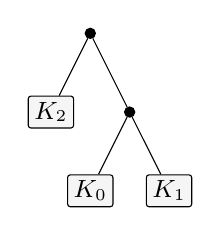
\begin{tikzpicture}[skeleton,level distance=10mm]
  \node[internal]{} child{node[atom]{$K_2$}} child{node[internal]{} child{node[atom]{$K_0$}} child{node[atom]{$K_1$}}};
\end{tikzpicture}
\hfill
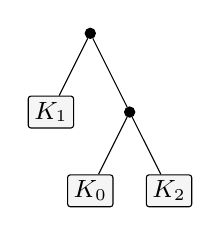
\begin{tikzpicture}[skeleton,level distance=10mm]
  \node[internal]{} child{node[atom]{$K_1$}} child{node[internal]{} child{node[atom]{$K_0$}} child{node[atom]{$K_2$}}};
\end{tikzpicture}
\hfill
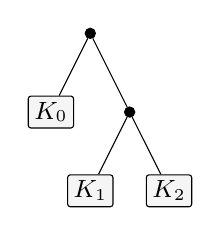
\begin{tikzpicture}[skeleton,level distance=10mm]
  \node[internal]{} child{node[atom]{$K_0$}} child{node[internal]{} child{node[atom]{$K_1$}} child{node[atom]{$K_2$}}};
\end{tikzpicture}\\[3mm]
leave $K_2$ at the root\qquad
leave $K_1$ at the root\qquad
leave $K_0$ at the root
\end{center}
Each tree has two asymmetric binary nodes and class size $2^2=4$.  Thus $N_{\min}=3$.  The Fuss--Catalan value $C_6=132$ gives $132/2^2=33\equiv1\pmod2$, agreeing with $(-1)^2/(1!1!1!)\equiv1$.  Corollary~\ref{cor:exact-count} also gives $4!/(2!\,2^2)=3$.
\end{example}

\begin{example}[Ternary trees: $(p,k,n)=(3,1,8)$]\label{ex:ternary}
Now $m=17=9+2\cdot3+2\cdot1=122_3$, so $t=(5-1)/(3-1)=2$ and the atoms are $K_0,K_0',K_1,K_1',K_2$.  Corollary~\ref{cor:exact-count} gives
\[
 N_{\min}=\frac{6!}{2!\,3^2\,(2!\,2!\,1!)}=10.
\]
Two of the ten skeletons, using distinct labels for equal-height atoms, are
\begin{center}
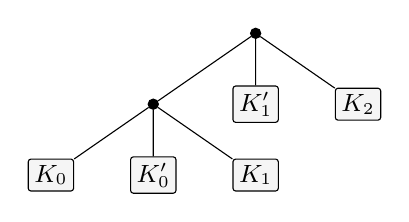
\begin{tikzpicture}[skeleton,sibling distance=13mm]
  \node[internal]{}
    child{node[internal]{} child{node[atom]{$K_0$}} child{node[atom]{$K_0'$}} child{node[atom]{$K_1$}}}
    child{node[atom]{$K_1'$}}
    child{node[atom]{$K_2$}};
\end{tikzpicture}
\qquad
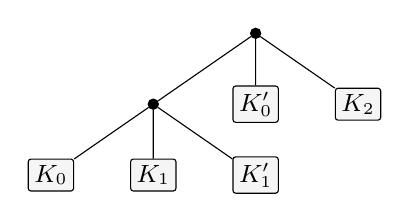
\begin{tikzpicture}[skeleton,sibling distance=13mm]
  \node[internal]{}
    child{node[internal]{} child{node[atom]{$K_0$}} child{node[atom]{$K_1$}} child{node[atom]{$K_1'$}}}
    child{node[atom]{$K_0'$}}
    child{node[atom]{$K_2$}};
\end{tikzpicture}
\end{center}
Both pictured cherries contain a repeated height, so as unlabelled skeletons each cherry has a single cyclic order, and each pictured choice of atoms gives two skeletons, which differ by the cyclic order of the three children of the root.  Sorting the ten skeletons by the two atoms that sit at the root next to the internal node: $\{K_0,K_0\}$ and $\{K_1,K_1\}$ give one skeleton each; $\{K_0,K_2\}$ and $\{K_1,K_2\}$ give two each; $\{K_0,K_1\}$ gives four (two cyclic orders at the root times two for the cherry $K_0,K_1,K_2$).  In all $1+1+2+2+4=10$.  Since $k=1$, all atoms are in one depth class and the vector is $(5)$.  Distinct labelling yields $T(5)=10(2!2!)=40$.  Two applications of the carry congruence give
\[
 T(5)\equiv-T(5-3+1)=-T(3)\equiv T(1)\pmod3,
\]
so $T(5)\equiv1\pmod3$, as $40$ confirms.  Here $C_8^{(3)}=43263$, $43263/3^2=4807$, and $4807\equiv1\pmod3$.  Theorem~\ref{thm:main} predicts $(-1)^2/(2!2!1!)=4^{-1}\equiv1\pmod3$.
\end{example}

\begin{example}[Quaternary trees: $(p,k,n)=(2,2,4)$]\label{ex:quaternary}
In this case $q=4$ and $m=13=8+4+1=1101_2$, so $t=2$, with atoms $K_0,K_2,K_3$.  Condition (S) is now essential: at depth $r$,
\[
 K_0\text{ and }K_2\text{ require }r\equiv0\pmod2,
 \qquad K_3\text{ requires }r\equiv1\pmod2.
\]
A binary cyclic skeleton with two internal nodes has two leaves at depth $2$ and one leaf at depth $1$.  Therefore $K_3$ must be the leaf adjacent to the root, while $K_0$ and $K_2$ form the cherry at depth $2$:
\begin{center}
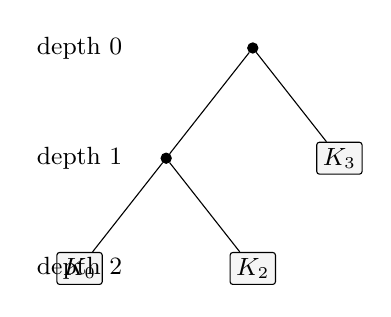
\begin{tikzpicture}[skeleton,level distance=14mm,sibling distance=22mm]
  \node[internal]{}
    child{node[internal]{} child{node[atom]{$K_0$}} child{node[atom]{$K_2$}}}
    child{node[atom]{$K_3$}};
  \node at (-2.2,0) {\small depth $0$};
  \node at (-2.2,-1.4) {\small depth $1$};
  \node at (-2.2,-2.8) {\small depth $2$};
\end{tikzpicture}
\end{center}
After atom expansion, the leaves of $K_0$ are at depth $2$, those of $K_2$ at depth $2+2=4$, and those of $K_3$ at depth $1+3=4$.  All these depths are even, as required for $q=4$.  There is one minimal class.

For a labelled illustration of carrying, classes $0$ and $1$ in $\Z_2$ give the vector $\mathbf a=(2,1)$, since $K_0,K_2$ are labels of class $0$ and $K_3$ is of class $1$.  First carry the two class-$0$ labels, then the two resulting class-$1$ labels:
\[
 (2,1)\longrightarrow(0,2)\longrightarrow(1,0).
\]
Modulo $2$, the carry congruence reads $T(\mathbf a)\equiv-T(\mathbf a')\equiv T(\mathbf a')$.  Thus
\[
 T(2,1)\equiv-T(0,2)\equiv T(1,0)\pmod2.
\]
The actual values are all $1$, and $N_{\min}=1$.  Indeed $C_4^{(4)}=140$ and $140/2^2=35\equiv1\pmod2$.
\end{example}

\begin{thebibliography}{9}
\bibitem{Konvalinka}
Matja\v{z} Konvalinka, ``Divisibility of generalized Catalan numbers'', \emph{Journal of Combinatorial Theory, Series A} \textbf{114} (2007), no.~6, 1089--1100. DOI: \href{https://doi.org/10.1016/j.jcta.2006.11.003}{10.1016/j.jcta.2006.11.003}.

\bibitem{DeutschSagan}
Emeric Deutsch and Bruce E. Sagan, ``Congruences for Catalan and Motzkin numbers and related sequences'', \emph{Journal of Number Theory} \textbf{117} (2006), no.~1, 191--215. DOI: \href{https://doi.org/10.1016/j.jnt.2005.06.005}{10.1016/j.jnt.2005.06.005}.

\bibitem{PostnikovSagan}
Alexander Postnikov and Bruce E. Sagan, ``What power of two divides a weighted Catalan number?'', \emph{Journal of Combinatorial Theory, Series A} \textbf{114} (2007), no.~5, 970--977. DOI: \href{https://doi.org/10.1016/j.jcta.2006.09.007}{10.1016/j.jcta.2006.09.007}.

\bibitem{KerstingFischer}
Sophie Johanna Kersting and Mareike Fischer, ``Measuring tree balance using symmetry nodes --- A new balance index and its extremal properties'', \emph{Mathematical Biosciences} (2021). DOI: \href{https://doi.org/10.1016/j.mbs.2021.108690}{10.1016/j.mbs.2021.108690}. arXiv:2105.00719.

\bibitem{Etherington}
I. M. H. Etherington, ``On non-associative combinations'', \emph{Proceedings of the Royal Society of Edinburgh} \textbf{59} (1940; issued separately 1939), 153--162. DOI: \href{https://doi.org/10.1017/S0370164600012244}{10.1017/S0370164600012244}.
\end{thebibliography}
\end{document}
